\section{Design}

Review and evaluation of Ohmage reference application and open mHealth schema.
Review case studies. 
Design and prototype alternative trust / security approach to current OAuth2-based mechanism. 
Design new repository. 
Provide NDN-CCL and NFD support for Android. 
Trying replacing REST backend in Ohmage with NDN.


\paragraph{Approach}
Follow up on mHealth design approach from Estrin \& Sim, 2010.
Use Ohmage as a reference application. 

Plan to create/port a mobile client for the Ohmage reference platform, which currently incorporates:
Mobile application, LAMP stack back-end, REST communication

Key pain point is OAuth 2.0:  Implementation relies on this � doesn�t scale to the DPU model and has numerous problems.  Quickly identified by 

Open mHealth lead architect as a primary challenge.   

Same approach (apparently) used in Human API mentioned earlier. 

Capture (Anyang / Tsinghua / UCLA) 
Storage (Tsinghua / UCLA)
Processing (Basel)
Presentation (REMAP)
Security (Michigan)

\paragraph{Design Goals} 

\begin{itemize}
\item \textbf{Interoperable, Internet-inspired data exchange} as the backbone of the application ecosystem
\item \textbf{Thin waist of open data interchange standards} that will enable an ecosystem of sensing, storage, analysis, and user interface components to support medical discovery and evidence-based care 
\item Market-supported, patient-centered landscape of innovative health applications
\item \textbf{Patient-controlled, privacy-aware data exchange} across device, component, and application boundaries
\end{itemize}


\paragraph{What to keep from current Open mHealth design.}
\begin{itemize}
\item Data-centric rather than service-centric interoperability. $\Rightarrow$ \emph{Focus on data namespace design.}
\item Distributed architecture of Capture, DSU, DPU, DVU. $\Rightarrow$ \emph{Implement data flow approach in NDN.}
\item End user focus (not hospitals, doctors, etc.) $\Rightarrow$ \emph{Consumer app deployment scenario.}
\item User-centric privacy approach. $\Rightarrow$ \emph{Need to inform user of choices, data flow.}
\item Encrypted communications. $\Rightarrow$ \emph{Encryption-based access control, name encryption.}
\item Mobile publishing. $\Rightarrow$ \emph{Use as our driver to solve this oft-cited challenge.}
\end{itemize}

\paragraph{What to discard from current Open mHealth design.}
\begin{itemize}
\item REST/HTTP: Move away from RPC call model and carrying state in Interests.
\item Host-based endpoints for services:  focus on data dissemination model and NFN style processing. 
\item OAuth: need new identity / authentication support. 
\item Single storage ``location''. 
\end{itemize}

\paragraph{mHealth Reality Check}

%% From 
%% PLOS Medicine Editors. "A reality checkpoint for mobile health: three challenges to overcome." PLoS Medicine 10.2 (2013).
%% TODO: Add to cites

\begin{itemize}
\item \textbf{Are your systems interoperable?}
Estrin \& Sim in Science, 2010.  Open mHealth. 
\item \textbf{Are you using open standards?}
WHO, 2013.  eHealth unit. 
\item \textbf{How will you evaluate?}
Greenhalgh et al. in BMC Med Res. Methodology, 2011.
Realist and meta-narrative evidence synthesis.
\end{itemize}

\subsection{NDNEx Application components}

Translate existing REST-based approach?  How quickly to move to a new model of data exchange where transactions are mostly about (for example) keys. 

Based on 
PEIR, the personal environmental impact report, as a platform for participatory sensing systems research. Mun, M., Reddy, S., Shilton, K., Yau, N., Burke, J., Estrin, D., ... \& Boda, P. (2009, June). Proc. ACM Mobisys 2009. 


User interacts with three pieces:
\begin{itemize}
\item Mobile capture application
\item Website for visualization / review
\item Identity manager
\end{itemize}

%%%%%%%%%%%%%%

\subsubsection{Mobile capture}

One of two primary user interfaces. 

Design for Android. Port NFD, tools.

We are going to use the Ohmage Android client (including the Mobility module) with only the in-app storage and communication changed to NDN. 
See (Tangmunarunkit, H., et al., 2014) and also the papers on the Ohmage website. 

Note that Mobility generates activity classified data that may not require the Activity Classification DPU in the initial version.

Instance of TCP/IP Ohmage (client and server) is now up and running thanks to Haitao in Lixia�s group at UCLA.  

Initial analysis of Ohmage mobile client communication completed by Prof. Euihyun Jung�s group from Anyang Univ.   

From Basel: Today, we had an internal presentation from the Psychology Dept which explained their use of the Ohmage system that is running in Basel. Although NDNex comes too late for being applied in ongoing projects, these projects are a good source of insights about user requirements for our future NDNex system, especially the aspect of data sovereignty.


\subsubsection{Building Block: Ohmage \& Mobility}

\url{http://ohmage.org/}

ohmage is an open-source participatory sensing technology platform. It supports: 1) expressive project authoring; 2) mobile phone-based data capture through both inquiry-based surveys and automated data capture as well as temporally and/or spatially triggered reminders, 3) data visualization and real-time feedback; privacy respecting data management; and 4) extensible data exploration. 

Tangmunarunkit, H., et al. "Ohmage: A General and Extensible End-to-End Participatory Sensing Platform,� ACM Trans. on Intelligent Systems and Technology (in submission), UCLA CS Technical Report 140015. (Used in 20 projects.)  \url{http://web.ohmage.org/~hongsudt/pub/ohmage_ucla_140015.pdf}


%%%%%%%%%%%%%%

\subsubsection{Data Storage}

Approach:  One or more new NDN repo designs supporting a hierarchy of storage needs: mobile device, user private repository, temporary processing storage.

Requirements: From Open mHealth Data Storage Unit (DSU) Design and overall application architecture.

Storage at:
\begin{itemize}
\item The mobile device itself.
\item A personal data repository (which may be distributed).
\item Temporary storage for processing and visualization components. 
\end{itemize}

Current plan:  implement in Java using jNDN, for Android support. 

Design led by Jianxun in Dan Pei�s group at Tsinghua. 

\paragraph{Reference: Open mHealth Data Storage Unit (DSU) Design}

\url{https://github.com/openmhealth/developer/wiki/DSU-Overview}

The Open mHealth DSU (Data Storage Unit) API Specification is an open specification for unified information sharing across disparate data streams. The idea is simple: create an easy-to-understand set of APIs that allow siloed data stores to share information. Third-party applications that understand this API specification can then create a single set of tools to access data across any of the servers.

\paragraph{Building Block: Personal Data Vault}
Reference Derek's work here? 

Mun, Min, et al. "Personal data vaults: a locus of control for personal data streams." Proceedings of the 6th International Conference. ACM, 2010.http://remap.ucla.edu/jburke/publications/Mun-et-al-2010-Personal-Data-Vaults.pdf

Kang, J., Shilton, K., Estrin, D., Burke, J. "Self-surveillance privacy." Iowa L. Rev. 97 (2011): 809.http://escholarship.org/uc/item/1jk8b2q1.pdf



%%%%%%%%%%%%%%

\subsubsection{Processing}

Goal here is to have a few representative components implemented using NFN-style approach, not exactly the processing blocks listed above, necessarily.  

Ideally, provide composable data flow inspired by Google Cloud Dataflow, Apache Spark, etc.  

Start with GeoFencing, as activity classification is currently handled in the Mobility portion of Ohmage.  But, could also consider other application-specific processing ideas. 

Web-based front end using NDN-JS with access to geofenced location information, providing location-specific content back to the mobile user.

Related to vehicular networking work. 

\paragraph{Reference: Open mHealth Data Processing Unit (DPU) Design}

\url{https://github.com/openmhealth/developer/wiki/Open-mHealth-and-Data-Processing}

DPUs are stateless modules that input and output data. They are designed to be embedded in other software or called remotely. They do not produce anything directly visible, but are the brains and muscles of an application. The concept of a DPU is inspired by the Unix Philosophy of creating small functional tools that can be chained and reused, rather than a single large application.

\paragraph{Building Block: Named Function Networking }

\url{http://www.named-function.net/}

Names serve to access and invoke functions, which incidentally can produce passive content once it is needed. New questions arise from this point of view, namely how the network organizes the flow of functions, which brings us squarely into active networking turf. 

Initially, focusing on location-based triggers (geofencing) - to trigger location-based content.

\subsubsection{Content Source: Trails Database}

\url{http://archinect.com/news/article/111897927/tour-los-angeles-history-with-ucla-s-new-interactive-urban-trail-app}

The LASHP Trails Mobile Website gives residents and visitors to Northeast Downtown Los Angeles site-specific access to a dynamic combination of historic information and health-related activities along urban trails starting and ending at the Los Angeles State Historic Park. 


%%%%%%%%%%%%%%

\subsubsection{Visualization}
Start with Ohmage web front end
And Lifestreams?
NDN-JS and D3
Web-based front end using NDN-JS with access to geofenced location information, providing (for example) running trail visualization.
Perhaps use many GPX format visualizers.  E.g., \url{http://flowingdata.com/2014/02/05/where-people-run/}

Web-based front end using NDN-JS to access derived data without location information.
Examples: http://quantifiedself.com/fitbit/   


\paragraph{Reference: Lifestreams Dashboard}

\cite{hsieh2013acm}

\paragraph{Building Block: Analytics / Presentation: Ohmage Front-end for Mobilize}

\url{https://wiki.mobilizingcs.org/app/web}

The web frontend (powered by the ohmage project) is used to provide students secure access to their data. It supports secure login, campaign management, data management and basic campaign monitoring and visualization. The students can review and share their data to the growing data set collected by their class. The web frontend can also be used to discover the answers to basic statistical inferences in real-time as data is being collected. When data collection is complete, the web frontend allows for easy exporting of the data to a more thorough statistical analysis tool. 



%%%%%%%%%%%%%%

\subsubsection{Identity Manager}
  
  
  
  
%%%%%%%%%%%%%%
  
\subsection{Trust and security}

Replacing Oauth2 for distributed processing is critical
One
entity (here, the `` user") maintains multiple publishers whose data are
consumed by many services with varying levels of access based on the: type
of data (as expressed in the name), level of granularity, and date/time
when the data was produced. ABE seems a good fit here, is it viable for
practical experimentation or do we need a directory-of-symmetric-keys or
some other approach?  If not ABE, where should we begin for our approach?
Are there existing best practices?


\subsubsection{Trust model} 
Leverage PKI as deployed
Would like to start from the same tools being used for user/gateway trust management in NDN testbed for this application.  
How to take advantage of the NDN signing infrastructure?
Certificates and delegation of authority.

\subsubsection{Identity}
Each processing block in this diagram may come from a different service provider. 
User may have different identity per service (or at least per flow). 
Each step tends to generate derived data that must also be stored and may not be associated with the original identity.  

We are exploring the idea of an ``identity manager", an application
manages the certificates (identities) that an individual uses to interact
with the various services involved in this application. Are there good
examples of \emph{user interfaces} for identity management already?  In fact,
pointers to state-of-the-art in end-user interfaces for security decision
making would be helpful. Alex doesn't think there are many. 

\subsubsection{Integrity} 

\subsubsection{Confidentiality}

Principal of minimum information. 

Access control in "data flow" model for communication between processing components, replacing Oauth (with Tsinghua and UCLA).  Extensions to support epidemiological studies incorporating semi-anonymized opt-in data across large populations. 

We will need to come up with an approach for name encryption for
this environment, in a way that still enables applications to operate on
the namespace--perhaps without having to be concerned with
decryption--once it has been decrypted and/or de-encapsulated.


\subsubsection{Data flow model support}
We imagine a data flow like model for this system:
[Publisher]->[Processing]->[Processing]->[Visualization], with each []
block being owned by a different entity and an objective to leak the
minimum amount of context to the processing components.  I'm not sure we
understand how to handle authentication /  access control of the
intermediate processing blocks, to each other and to the source/sink of
the data.  Where can we look for best practices for security in current
data flow architectures?

%%%%%%%%%%%%%%
  

\subsection{Naming}

\subsubsection{Data}
Personal health data (and metadata) namespace and repository design � focusing on support for physical activity data in the first round.  
What schema? Initially, try direct mapping of Open mHealth schema to names


\textbf{Basis of design}: Open mHealth Physical Activity data schema\footnote{\url{http://www.openmhealth.org/developers/schemas/#physical-activity} and \url{http://bioportal.bioontology.org/ontologies/SNOMEDCT?p=classes&conceptid=68130003}}, as well as other schemas from Open mHealth as needed. 

\begin{listing}
\begin{minted}[frame=single,
               framesep=3mm,
               linenos=false,
               fontsize=\footnotesize,
               tabsize=2]{js}
{     
    "$schema": "http://json-schema.org/draft-04/schema#",

    "description": "This schema represents a single episode of physical activity.",
    "type": "object",
    "references": [
        {
            "description": "The SNOMED code represents Physical activity (observable entity)",
            "url": "http://purl.bioontology.org/ontology/SNOMEDCT/68130003"
        }
    ],
    "definitions": {
        "activity_name": {
            "$ref": "activity-name-1.0.json"
        },
        "length_unit_value": {
            "$ref": "../generic/length-unit-value-1.0.json"
        },
        "time_frame": {
            "$ref": "../generic/time-frame-1.0.json"
        }
    },

    "properties": {
        "activity_name": {
            "$ref": "#/definitions/activity_name"
        },
        "effective_time_frame": {
            "$ref": "#/definitions/time_frame"
        },
        "distance": {
            "description": "The distance covered, if applicable.",
            "$ref": "#/definitions/length_unit_value"
        },
        "reported_activity_intensity": {
            "description": "Self-reported intensity of the activity performed.",
            "type": "string",
            "enum": ["light", "moderate", "vigorous"]
        }
    },

    "required": ["activity_name"]
}
\end{minted}
\caption{Open mHealth Physical Activity Schema, retrieved December 28, 2014. See appendix for subschema.} 
\label{listing:physical-activity-json}
\end{listing}




How to separate this into namespace and data?
Figure~\ref{fig:ndnex-namespace}

JSON payload. 

\begin{figure}
\begin{center}
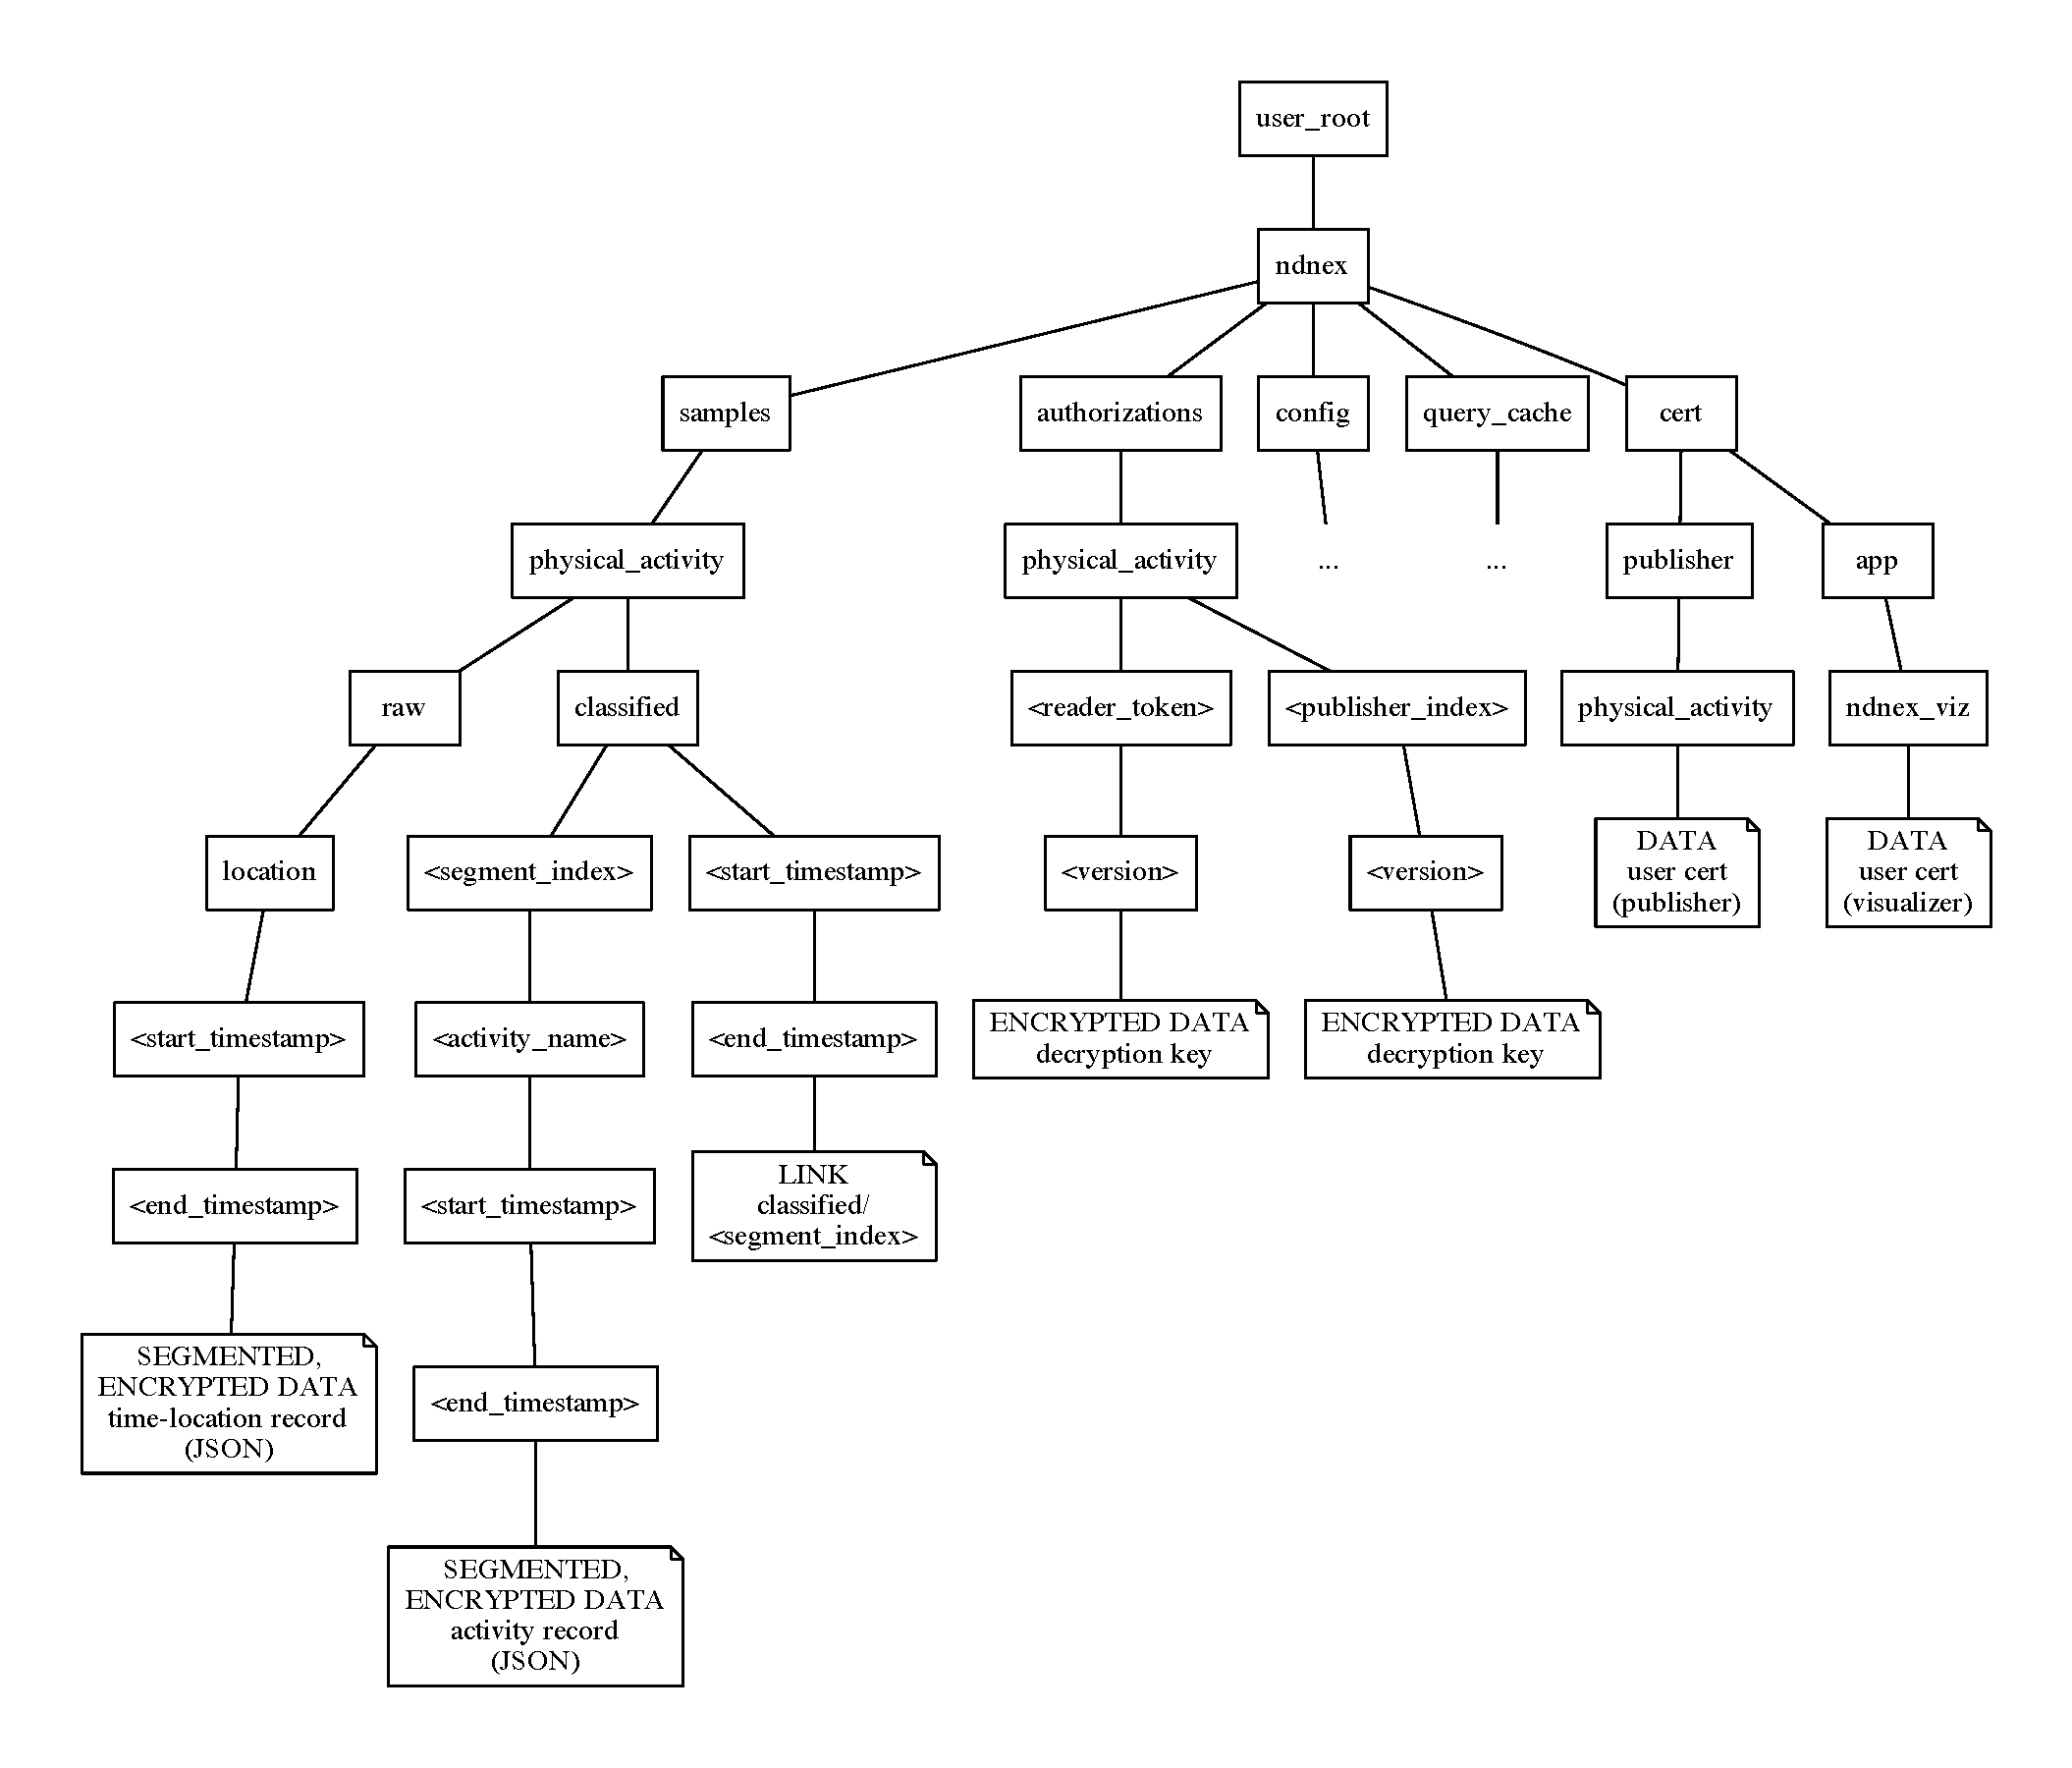
\includegraphics[width=1\textwidth]{figures/ndnex-name-top-01}
\caption{NDNEx Namespace, version 1.}
\label{fig:ndnex-namespace}
\end{center}
\end{figure}

\subsubsection{Certificates}

\subsubsection{Processing}
Borrow ideas from Named Function Networking concept for distributed processing

%%%%%%%%%%%%%%
  

\subsection{Storage}

A distributed network of repos replaces the ecosystem of DSUs envisioned in the Open mHealth TCP/IP architecture. 

(Hierarchical network of repositories, similar to BAS/BMS, including both personal repositories, service provider backups for personal data, and aggregated "anonymized" stores). 

Write access control

A mechanism for delegating authority to publish into a repository is
necessary. 
\subsection{Routing \& Forwarding}
Mobile publishing support



\begin{figure}
\centering
\subfigure[Mobile publisher connected to ``home'' hub, which directly routes its publishing prefix.]{
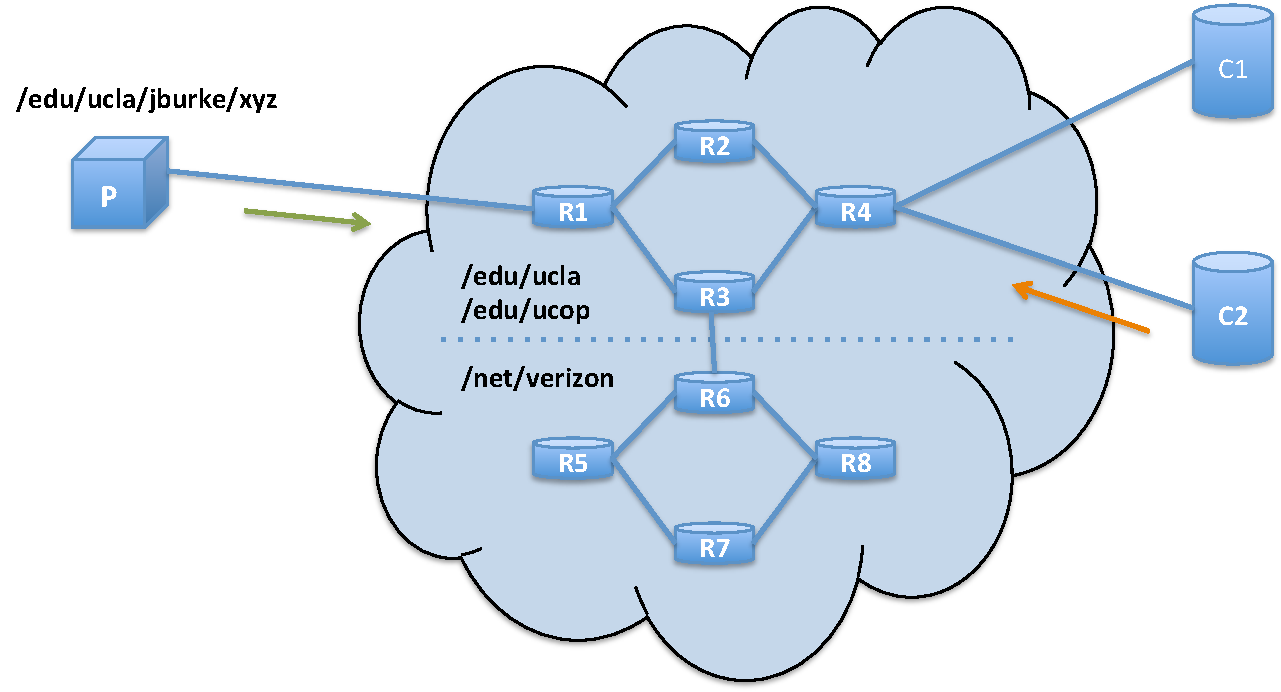
\includegraphics[width=0.45\columnwidth, keepaspectratio=true]{figures/publisher-mobility-a}
}
\subfigure[Mobile publisher connected to another hub, which does not directly route its prefix.]{
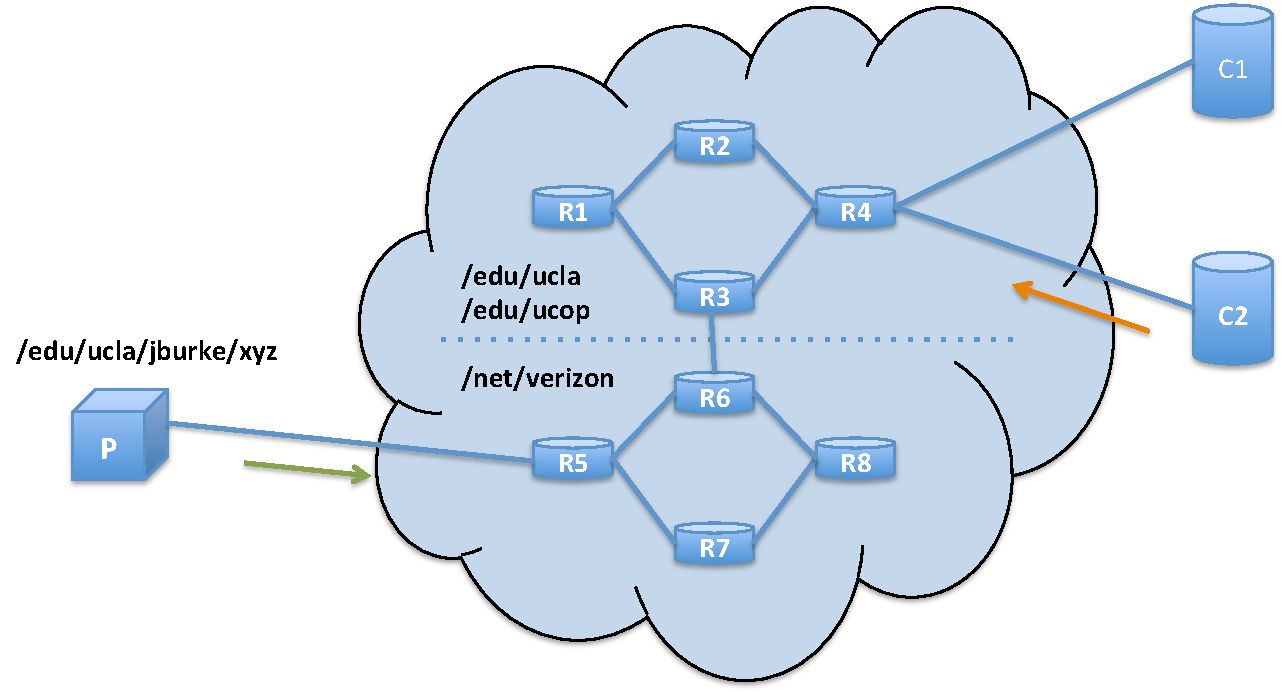
\includegraphics[width=0.45\columnwidth, keepaspectratio=true]{figures/publisher-mobility-b}
}
\caption{Mobile publisher scenario.}
\label{fig:mobilepublisher}
\end{figure}

\subsection{Distributed Processing}
Incorporate Haitao's design?
Named Function Networking style support for distributed processing with University of Basel. 




